\chapter{Fluid Mechanics}

The motion of a fluid is completely described by the conservation laws for the three basic properties: mass, momentum and energy.
Indeed,how complicated the detailed evolution of a system might be, not only are the basic
properties mass, momentum and energy conserved during the whole process at all
times but more than that, these three conditions
completely determine the behavior of the system without any additional dynamical
law.
This is a very remarkable property, indeed. The only additional information
concerns the specification of the nature of the fluid (e.g. incompressible fluid, perfect
gas, condensable fluid, viscoelastic material, etc.).
A fluid flow is considered as known if, at any instant of time, the velocity field
and a minimum number of static properties are known at every point. The number of
static properties to be known is dependent on the nature of the fluid. This number will
be equal to one for an isothermal incompressible fluid (e.g. the pressure), two (e.g.
pressure and density) for a perfect gas or any real compressible fluid in thermodynamic
equilibrium.

We will consider that a separate analysis has provided the necessary knowledge
enabling to define the nature of the fluid. This is obtained from the study of the behavior
of the various types of continua and the corresponding information is summarized
in the constitutive laws and in some other parameters such as viscosity and heat
conduction coefficients. This study also provides the information on the nature and
properties of the internal forces acting on the fluid since, by definition, a deformable
continuum such as a fluid, requires the existence of internal forces connected to the
nature of the constitutive law.
Besides, separate studies are needed in order to distinguish the various external
forces that influence the motion of the system in addition to the internal ones. These
external forces could be, e.g. gravity, buoyancy, Coriolis and centrifugal forces in
rotating systems, electromagnetic forces in electrical conducting fluids.

Let us now move to the derivation of the basic fluid dynamic equations, by
applying the general expressions derived in the previous chapter, to the specific quantities
mass, momentum and energy.
The equation for mass conservation is also called the continuity equation, while the
momentum conservation law is the expression of the generalized Newton law, defining
the equation of motion of a fluid. The energy conservation law is also referred to as
the expression of the first principle of Thermodynamics.


\newpage
\section{Forms of the Fundamental Equations}
Vorticity $\vec{\omega}$
\begin{equation}
    \label{vorticity}
    \Omega_i \defeq e_{ijk}\frac{\partial v_k}{\partial x_j}  \defeq  \left( \nabla \times \vec{v} \right)_i 
\end{equation}

Circulation $\Gamma$
\begin{equation}
    \label{circulation}
    \Gamma \defeq \oint v_i dx_i  \defeq \oint \vec{v} d\vec{x}
\end{equation}



\newpage
\section{Navier-Stokes Flow}

\subsection*{Mass:}

\subsection*{Momentum:}

\subsection*{Energy:}







\newpage
\section{Thin Shear Layers Flow}

\subsection{Boundary Layer Flow}








\newpage
\section{Euler Flow}
The Euler flow can be taken directly from the fundamental equations of chapter \ref{fundamentals}, however they are derivable from the Navier-Stokes flow equation by assuming that there are no viscous/shear forces present i.e. $\tau_{ij}=0$.
\subsection*{Mass:}
\begin{equation}
    \frac{\partial \rho}{\partial t} +  \frac{\partial \rho v_j}{\partial x_j} = 0
\end{equation}

\subsection*{Momentum:}
\begin{equation}
    \frac{\partial \rho v_i}{\partial t} +  \frac{\partial \rho v_i v_j}{\partial x_j} = \rho f_i - \frac{\partial p}{\partial x_i}
\end{equation}

\subsection*{Energy:}
\begin{equation}
    \frac{\partial \rho e_u+ \rho\frac{v_i v_i}{2}}{\partial t} +  \frac{\partial (\rho e_u + \rho\frac{v_i v_i}{2} v_j)}{\partial x_j} =  \dot{q} + \frac{\partial} {\partial x_j} \left( k\frac{\partial T}{d x_j} \right) - \rho f_i v_i  + \frac{\partial  p v_j }{\partial x_j}
\end{equation}


\subsection{Steady Quasi-1D Adiabatic Euler Flow}




\subsection{Steady 1D Adiabatic Euler Flow}
\label{1d_adiabatic_inviscid}
An case of extreme engineering importance is the Euler flow equations for a steady, uni-dimensional and adiabatic produces the following simplified equations.
This situation can be used to explain properties of flows in supersonic conditions, and their shock waves.
\hl{talk about what means 1D vs Quasi 1D}

\subsubsection*{Mass:}
\begin{align}
    \int\limits_{\mathcal{A}} \rho v_j n_j dA &= 0 \\
    \rho_1 v_1  &=\rho_2 v_2
\end{align}

\subsubsection*{Momentum:}
\begin{align}
    \int\limits_{\mathcal{A}} \rho v_i v_j n_j dA &= \int\limits_{\mathcal{A}} - p n_i dA \\
    \rho_1 v^2_1 + p_1&=  \rho_2 v^2_2 + p_2
\end{align}

\subsubsection*{Energy:}
\begin{align}
    \int\limits_{\mathcal{A}} (\rho u + \rho\frac{v_i v_i}{2}) v_j n_j dA &= \int\limits_{\mathcal{A}} - p v_j n_j dA \\
    \rho_1 e_{I_1} + \rho_1\frac{v^2_1 }{2} v_1  + p_1 v_1 &= \rho_2 e_{I_2} + \rho_2\frac{v^2_2 }{2} v_2 +  p_2 v_2
\end{align}

\subsubsection{Normal Shock Waves}
the mach numbers after $M_2$ and before $M_1$, are related between themselves by:
\begin{equation}
    M_2^2=\frac{1+ \frac{\gamma -1}{2}M_1^2}{\gamma M_1^2 - \frac{\gamma -1}{2}}
\end{equation}
While the pressure, density, velocity, temperature and entalpy ratios across the normal shock are given by:
\begin{align}
    \frac{p_2}{p_1} &= 1+\frac{2\gamma}{\gamma +1} \left(M_1^2-1 \right)\\
    \frac{\rho_2}{\rho_1} &= \frac{v_1}{v_2}=\frac{\left(\gamma+1 \right) M_1^2}{2+\left(\gamma -1 \right) M_1^2}\\
    \frac{T_2}{T_1} &= \frac{p_2}{p_1}=\frac{\rho_1}{\rho_2}=\frac{h_2}{h_1}
\end{align}

This resumes the fundamental equations for the calculation of flows properties across normal shock waves.
\subsubsection{Oblique Shock Waves}


\subsubsection{Prandtl-Meyer Expansion Waves}

The expansion waves are the opposite of shock waves, hence trough an expansion wave the Mach number increases and pressure, density and temperature decreases.

The expansion fan is itself a continuous expansion region, composed of an infinite number of Mach waves, bounded upstream and downstream.
The all expansion is composed of infinitesimal Mach waves we can consider the process isentropic, all the way through the wave, and therefore the stagnations relations are applicable.



\begin{equation}
\nu(M)=\sqrt{\frac{\gamma +1}{\gamma-1}} \tan^{-1}\left( \sqrt{\frac{\gamma -1}{\gamma+1}(M^2-1)} \right) -\tan^{-1} \left( \sqrt{M^2-1}\right)
\end{equation}
\subsubsection{Interaction of Shock Waves}



\newpage
\subsection{Fanno Flow}
Adiabatic flow through a constant area duct where the effect of friction is considered is also know as Fanno flow.

\newpage
\subsection{Steady 1D Non-Adiabatic Euler Flow (Rayleigh Flow)}
Non-adiabatic flow through a constant area duct where the effect of heat addition or rejection is also know as the
Rayleigh. The only significant difference relative to the 1D adiabatic Inviscid Flow of \ref{1d_adiabatic_inviscid} is the addition of heat to the energy equation.
\subsubsection*{Mass:}
 \begin{align}
    \int\limits_{\mathcal{A}} \rho v_j n_j dA &= 0 \\
    \rho_1 v_1  &= \rho_2 v_2
\end{align}


\subsubsection*{Momentum:}
\begin{align}
    \int\limits_{\mathcal{A}} \rho v_i v_j n_j dA &= \int\limits_{\mathcal{A}} - p n_i dA \\
    \rho_1 v^2_1 + p_1&=  \rho_2 v^2_2 + p_2
\end{align}

\subsubsection*{Energy:}
\begin{align}
     \int\limits_{\mathcal{A}} (\rho u + \rho\frac{v_i v_i}{2}) v_j n_j dA &=  \int\limits_{\mathcal{V}} \dot{q} dV + \int\limits_{\mathcal{A}} - p v_j n_j dA \\
     \rho_1 e_{I_1} + \rho_1\frac{v^2_1 }{2} v_1  + p_1 v_1 &= q + \rho_2 e_{I_2} + \rho_2\frac{v^2_2 }{2} v_2 +  p_2 v_2
\end{align}

Solving the energy equation the heat per unit mass.
\begin{align}
     \rho_1 e_{I_1} + \rho_1\frac{v^2_1 }{2} v_1  + p_1 v_1 &= q + \rho_2 e_{I_2} + \rho_2\frac{v^2_2 }{2} v_2 +  p_2 v_2
\end{align}




% -------------------------------------------------POTENTIAL FLOW--------------------------------------------
\newpage
\section{Steady Incompressible Potential Flow}
The potential flow is definitely very important since, when further linearized, provides one of the only analytical methods of determining aerodynamic properties in airfoils and wing for either subsonic and supersonic.
We start by presenting flow equation, that are obtainable from the Euler flow by assuming no volumetric forces $\vec{f}=0$, adiabatic i.e. no heat transfers and constant density.

\subsection*{Mass:}
\begin{align}
    \label{mass_potential}
    \frac{\partial v_j}{\partial x_j} = 0 
\end{align}

\subsection*{Momentum:}
\begin{align}
    \label{momentum_potential}
    \rho \frac{\partial v_i v_j}{\partial x_j}= - \frac{\partial p}{\partial x_i}
\end{align}


\subsection*{Scalar Potential:}
The flow gains its name from the assumption that the flow velocity can be obtained from the gradient of scalar potential field $\phi$.
\begin{align}
    \label{scalar_potential}
    v_i \defeq  \frac{\partial \phi}{\partial x_i} = \left( \nabla \phi \right)_i
\end{align}

Replacing the \eqref{scalar_potential} into the the mass equation \eqref{mass_potential} we see that the scalar potential verifies as Laplace equation.
\begin{align}
    \frac{\partial}{\partial x_j} \left( \frac{\partial \phi}{\partial x_j} \right) &= 0 \nonumber  \\
    \frac{\partial^2 \phi}{\partial x_j^2} &= 0 \nonumber  \\
    \nabla^2 \phi &= 0
\end{align}

Replacing \eqref{scalar_potential} into the definition of vorticity \eqref{vorticity} we verify that a potential flow is irrotational.
\begin{align}
    \Omega_i &= e_{ijk}\frac{\partial}{\partial x_j} \left( \frac{\partial \phi}{\partial x_k} \right) \nonumber  \\
    \Omega_i &= e_{ijk}\frac{\partial^2 \phi}{\partial x_j \partial x_k} \nonumber \\ 
    \Omega_i &= 0  
\end{align}


\subsection*{Vector Potential:}
A vector potential $\vec{\Psi}$ can also be used to determine the flow velocity .
\begin{align}
    \label{vector_potential}
    v_i \defeq  e_{ijk} \frac{\partial \Psi_k}{\partial x_j} =  \left( \nabla \times \vec{\Psi} \right)_i
\end{align}

Replacing the \eqref{vector_potential} into the the mass equation \eqref{mass_potential} is immediately verified.
\begin{align*}
    \frac{\partial}{\partial x_i} \left( e_{ijk} \frac{\partial \Psi_k}{\partial x_j}  \right) &= 0 \nonumber  \\
    e_{ijk} \frac{\partial^2 \Psi_k}{\partial x_i \partial x_j}  &= 0 \nonumber  \\
    0 &= 0
\end{align*}

Replacing the \eqref{vector_potential} into the vorticity definition \eqref{vorticity}
\begin{align}
    \Omega_i &= e_{ijk}\frac{\partial}{\partial x_j} \left(e_{klm}\frac{\partial \Psi_m}{\partial x_l}  \right)  \nonumber \\
    \Omega_i &= e_{ijk}e_{klm}\frac{\partial^2 \Psi_m}{\partial x_j \partial x_l} \nonumber \\ 
    \Omega_i &= \left( \delta_{il}\delta_{jm} - \delta_{im}\delta_{jl} \right)\frac{\partial^2 \Psi_m}{\partial x_j \partial x_l}  \nonumber\\ 
    \Omega_i &= \frac{\partial^2 \Psi_j}{\partial x_j \partial x_i} -  \frac{\partial^2 \Psi_i}{\partial x_j \partial x_j} \nonumber \\ 
    \Omega_i &= \frac{\partial^2 \Psi_j}{\partial x_i \partial x_j} -  \frac{\partial^2 \Psi_i}{\partial x_j^2} = \left(\nabla \left(\nabla \cdot \vec{\Psi} \right) - \nabla^2\vec{\Psi} \right)_i 
    \label{vector_potential_irrot_cond}
\end{align}
So the vector potential $\vec{\Psi}$ must be chosen so that if a irrotatonal flow is desired then the right hand side of \eqref{vector_potential_irrot_cond} must be equate to zero.

In a more general 3 dimensional case, as shown by \cite{} , the vector potential can be written as function of two scalar fields, know as stream functions $\psi$ and $\chi$.
\begin{equation}
    \Psi_i = \psi \frac{\partial \chi}{\partial x_i} = \left(\psi \nabla \chi \right)_i
\end{equation}


For \textbf{2D Cartesian} the vector potential is then given by
\begin{align}
    \psi &= \psi(x,y) \\
    \chi &= z \\
    \vec{\Psi} &=  \begin{bmatrix} 0 &  0 &  \psi(x,y)\end{bmatrix} 
\end{align}

For \textbf{3D Axisymmetric} the vector potential is then given by
\begin{align}
    \psi &= \psi(x,y) \\
    \chi &= z \\
    \vec{\Psi} &=  \begin{bmatrix} 0 &  0 &  \psi(x,y)\end{bmatrix} 
\end{align}



\subsection*{Complex Potential:}
The potential flow can be easily manipulated in a more compact form, if we use a analytical complex function $W(z)$ as function of the potential $\phi(x,y)$ and of the stream function $\psi(x,y)$.
\begin{align}
    W(z) &= \phi  + i \psi \label{w_def} \qquad z \in  \mathbb{C} \\
    z &=  x + iy \label{z_def}  \qquad x,y \in \mathbb{R}
\end{align}
The differentials of \eqref{z_def} and \eqref{w_def}
\begin{align}
    dz &= dx + idy  \\
    dW &= \frac{\partial W}{\partial z}dz \\
    dW &= \frac{\partial W}{\partial z}(dx + idy) \\
    dW &= \frac{\partial W}{\partial z}dx + i\frac{\partial W}{\partial z}dy \\
\end{align}

However the Complex potential is also a function $W(z) = W(x,y)$ therefore it's differential can also be given by
\begin{align}
    dW &= \frac{\partial W}{\partial x}dx  +  \frac{\partial W}{\partial y}dy 
\end{align}
Therefore equating both differentials we reach the following equality.
\begin{align}
     \frac{\partial W}{\partial z}  &= \frac{\partial W}{\partial x}\\
     \frac{\partial W}{\partial z}  &= \frac{1}{i}\frac{\partial W}{\partial y} 
\end{align}
Summing both equations we reach what is called commonly as the Wirtinger complex differential operator over function $W$
\begin{align}
     \frac{\partial W}{\partial z}  &= \frac{1}{2} \left(\frac{\partial W}{\partial x} - i\frac{\partial W}{\partial y} \right)
\end{align}
However if we subtracted both equations we would obtain the following equality
\begin{align}
     \frac{\partial W}{\partial x} = - i\frac{\partial W}{\partial y}
\end{align}
Expanding the $x$ and $y$ differentials of $W$
\begin{align}
    \frac{\partial W}{\partial x} &= \frac{\partial \phi}{\partial x} + i\frac{\partial \psi}{\partial x} \\  
    \frac{\partial W}{\partial y} &=  \frac{\partial \phi}{\partial y} + i\frac{\partial \psi}{\partial y}  
\end{align}
Replacing back
\begin{align}
     \frac{\partial \phi}{\partial x} + i\frac{\partial \psi}{\partial x} &= - i\left( \frac{\partial \phi}{\partial y} + i\frac{\partial \psi}{\partial y}  \right) \\
     \frac{\partial \phi}{\partial x} + i\frac{\partial \psi}{\partial x} &= \frac{\partial \psi}{\partial y} - i\frac{\partial \phi}{\partial y} 
\end{align}
Thus we obtain what is know as the Cauchy-Rienman condition.
 \begin{align}
     \frac{\partial \phi}{\partial x} &= \frac{\partial \psi}{\partial y} \\
     \frac{\partial \phi}{\partial y} &= -\frac{\partial \psi}{\partial x} 
\end{align}


\newpage
\subsection{Complex Singularity Models}
In this section we present set of singular flows that can be compounded by linear superposition to form more complex flows.  
\subsubsection{Uniform Flow}
Complex Potential:
\begin{align}
    W(z) &= U z e^{-i\alpha} \\
    W(z) &= U r e^{i(\theta - \alpha)} \\
    W(z) &= U r \cos(\theta - \alpha) + i U r \sin(\theta - \alpha) 
\end{align}

Potential and Stream Functions:
\begin{equation}
    \begin{cases}
        \phi = U r \cos(\theta - \alpha)\\
        \psi = U r \sin(\theta - \alpha)
    \end{cases}
\end{equation}

Velocity:
\begin{equation}
    \frac{dW}{dz} =  U e^{-i\alpha}  = U \cos\alpha - iU\sin\alpha
\end{equation}
\begin{equation}
    \begin{cases}
        U_x = U \cos\alpha\\
        U_y = U \sin\alpha
    \end{cases}
\end{equation}

\begin{figure}[!h]
    \centering
    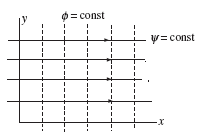
\includegraphics[scale=1.0]{./img/uniform_flow.png}
    \caption{Uniform flow with equipotential lines, and streamlines drawn.}
    \label{joukowski_cylinder}
\end{figure}

\subsubsection{Corner Flows}
Complex Potential:
\begin{align}
    W(z) &= A z^n
\end{align}




\subsubsection{Line of Sources}
Complex Potential:
\begin{align}
    W(z) &= \frac{Q}{2\pi}\ln(z-z_0) \\
    W(z) &= \frac{Q}{2\pi}\ln(r^*e^{i\theta^*}) \\
    W(z) &= \frac{Q}{2\pi}\left( \ln r^* + \ln(e^{i\theta^*}) \right) \\
    W(z) &= \frac{Q}{2\pi}\left( \ln r^* + i\theta^* \right)
\end{align}

Potential and Stream Functions:
\begin{equation}
    \begin{dcases}
        \phi = \frac{Q}{2\pi} \ln r^* \\
        \psi = \frac{Q}{2\pi} i\theta^*
    \end{dcases}
\end{equation}

Velocity:
\begin{equation}
    \frac{dW}{dz} =  \frac{Q}{2\pi} \frac{1}{z-z_0} = \frac{Q}{2\pi r^*} e^{-i\theta^*}
\end{equation}
\begin{equation}
    \begin{dcases}
        U_x = \frac{Q}{2\pi r^*}  \cos\theta^*\\
        U_y =  \frac{Q}{2\pi r^*}  \sin\theta^*
    \end{dcases}
    \Leftrightarrow
    \begin{dcases}
        U_r = \frac{Q}{2\pi r^*} \\
        U_{\theta} = 0
    \end{dcases}
\end{equation}

\begin{figure}[!h]
    \centering
    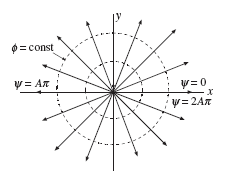
\includegraphics[scale=1.0]{./img/sourcesink_flow.png}
    \caption{Line of sources/sinks flow with equipotential lines, and streamlines drawn.}
    \label{joukowski_cylinder}
\end{figure}





\subsubsection{Line of Vortexes}
Complex Potential:
\begin{align}
    W(z) &= -\frac{i\Gamma}{2\pi}\ln(z-z_0) \\
    W(z) &= -\frac{i\Gamma}{2\pi}\ln(r^*e^{i\theta^*}) \\
    W(z) &= -\frac{i\Gamma}{2\pi}\left( \ln r^* + \ln(e^{i\theta^*}) \right) \\
    W(z) &= -\frac{i\Gamma}{2\pi}\left( \ln r^* + i\theta^* \right) \\
    W(z) &= \frac{\Gamma}{2\pi}\left( \theta^* - i\ln r^*\right)
\end{align}

Potential and Stream Functions:
\begin{equation}
    \begin{dcases}
        \phi = \frac{\Gamma}{2\pi} \theta^* \\
        \psi = - \frac{\Gamma}{2\pi} \ln r^*
    \end{dcases}
\end{equation}

Velocity:
\begin{equation}
    \frac{dW}{dz} =  \frac{i\Gamma}{2\pi} \frac{1}{z-z_0} = \frac{i\Gamma}{2\pi r^*} e^{-i\theta^*} = \frac{\Gamma}{2\pi r^*}\left(\sin\theta^* +i\cos\theta^* \right) 
\end{equation}
\begin{equation}
    \begin{dcases}
        U_x = \frac{\Gamma}{2\pi r^*}  \sin\theta^*\\
        U_y = -\frac{\Gamma}{2\pi r^*}  \cos\theta^*
    \end{dcases}
    \Leftrightarrow
    \begin{dcases}
        U_r = 0 \\
        U_{\theta} = -\frac{\Gamma}{2\pi r^*}
    \end{dcases}
\end{equation}

\begin{figure}[!h]
    \centering
    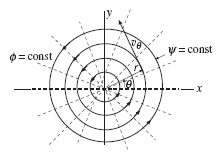
\includegraphics[scale=1.0]{./img/vortex_flow.png}
    \caption{Line of vortexes flow with equipotential lines, and streamlines drawn.}
    \label{joukowski_cylinder}
\end{figure}





\subsubsection{Line of Dipoles}
Complex Potential:
\begin{align}
    W(z) &= -\frac{\mu}{z} e^{i\alpha} \\
    W(z) &= -\frac{\mu}{r} e^{i(\alpha-\theta)} \\
    W(z) &= -\frac{\mu}{r} \left(\cos(\alpha-\theta) +i \sin(\alpha-\theta)  \right)
\end{align}

Potential and Stream Functions:
\begin{equation}
    \begin{dcases}
        \phi = -\frac{\mu}{r} \cos(\alpha-\theta) \\
        \psi = -\frac{\mu}{r} \sin(\alpha-\theta)
    \end{dcases}
\end{equation}

Velocity:
\begin{equation}
    \frac{dW}{dz} = \frac{\mu}{z^2} e^{i\alpha}  =  \frac{\mu}{r^2} e^{i(\alpha-2\theta)} = \frac{\mu}{r^2}\left( \cos(\alpha -2\theta) + i \sin(\alpha-2\theta) \right) 
\end{equation}
\begin{equation}
    \begin{dcases}
        U_x = \frac{\mu}{r^2}\cos(\alpha -2\theta) \\
        U_y = - \frac{\mu}{r^2}\sin(\alpha -2\theta)
    \end{dcases}
\end{equation}

\begin{figure}[!h]
    \centering
    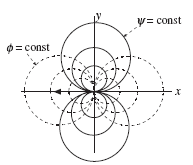
\includegraphics[scale=1.0]{./img/dipole_flow.png}
    \caption{Line of flow with equipotential lines, and streamlines drawn.}
    \label{joukowski_cylinder}
\end{figure}

\subsubsection{Line of Npoles}
Complex Potential:
\begin{align}
    W(z) &= -\frac{k}{z^{n-1}} 
\end{align}

Velocity:
\begin{equation}
    \frac{dW}{dz} = \frac{k}{z^{n}} 
\end{equation}
\

% \newpage
% \section{Aerodynamic Coefficients}
% \subsection{Pressure Coefficients}
% The pressure coefficient is the pressure difference from the local to the free stream, normalized for the dynamic pressure of the free stream.
% \begin{equation}
% C_p\defeq \frac{p - p_\infty}{\frac{1}{2} \rho_\infty v_\infty^2}
% \end{equation}

% Using the definition of the speed of sound, in conjunction with a isentropic process.

% \begin{equation}
% a^2=\left( \frac{\partial p}{\partial \rho} \right)_s = \gamma \frac{p}{\rho}
% \end{equation}

% An by the definition of number of Mach.
% \begin{equation}
% M \defeq \frac{U}{a}
% \end{equation}

% So we can rewrite the pressure coefficient for incompressible flows.

% \begin{equation}
% C_p=\frac{p - p_\infty}{\frac{1}{2}\gamma p_\infty M_\infty^2}=\frac{1}{\frac{1}{2}\gamma M_\infty^2}\left(\frac{p}{p_\infty} -1 \right)
% \end{equation}


% Using the isentropic relation relative to the estagnation point.

% \begin{equation}
% \frac{p_o}{p}=\left( 1 + \frac{\gamma -1}{2}M^2 \right)^{\frac{\gamma-1}{\gamma}}
% \end{equation}

% Keeping in mind that:

% \begin{equation}
% \frac{p}{p_\infty}=\frac{\frac{p_o}{p_\infty}}{\frac{p_o}{p}}
% \end{equation}

% So coefficient of pressure in terms of the local Mach number can be expressed by:

% \begin{equation}
% C_p=\frac{1}{\frac{1}{2}\gamma M_\infty^2} \left[ \left( \frac{1 + \frac{\gamma -1}{2}M_\infty^2}{1 + \frac{\gamma -1}{2}M^2}\right)^{\frac{\gamma-1}{\gamma}} -1 \right]
% \end{equation}



\newpage
\chapter{Airfoil Theory}

\section{Generalized Conformal Mapping}
In order to obtain the flow around airfoils, a set of transformations can be applied to the complex potential field.
In a general form these can be of the following type.
\begin{equation}
    \label{general_transform}
    z = \zeta + \sum\limits_{n=1} \frac{a_n}{\zeta^n}  \qquad \zeta, z, a_n \in \mathbb{C}
\end{equation}
The properties of these conformal transforms are quite interesting and provide powerful mechanisms to generate airfoil shapes.

\section{K\'arm\'an-Treftz Airfoils}
An airfoil family for which the Joukowski is actually a special case, is the K\'arm\'an-Trefetz transformations. 
\begin{equation}
    \label{karman_transform}
    z = kb \frac{(\zeta +b)^k + (\zeta -b)^k }{(\zeta +b)^k - (\zeta -b)^k }
\end{equation}
K\'arm\'an-Treftz Airfoils have some advantageous properties relative to the Joukowski airfoils, mainly the angle of the trailing edge. 
Since the trailing edge angle is different from the Joukowski $2\pi$ which is unfeasible to physically build.

\section{Joukowski Airfoils}
The Joukowski airfoil can be derived from the general transform \eqref{general_transform} using $a_1 = b \vee a_n = 0$ with  $n \geq 2$. Or from the
K\'arm\'an-Treftz transform \eqref{karman_transform} with $k=2$.
\begin{equation}
    \label{joukowski_transform}
    z = \zeta + \frac{b^2}{\zeta} 
\end{equation}
The Joukowski airfoil has very interesting properties since a circle in the $\zeta$ plane will transform into an airfoil in the $z$ plane.
The geometrical properties of this airfoil will be determined, has we shall seen, on the offset from the center of the $\zeta$ plane origin.
\begin{figure}[!h]
    \centering
    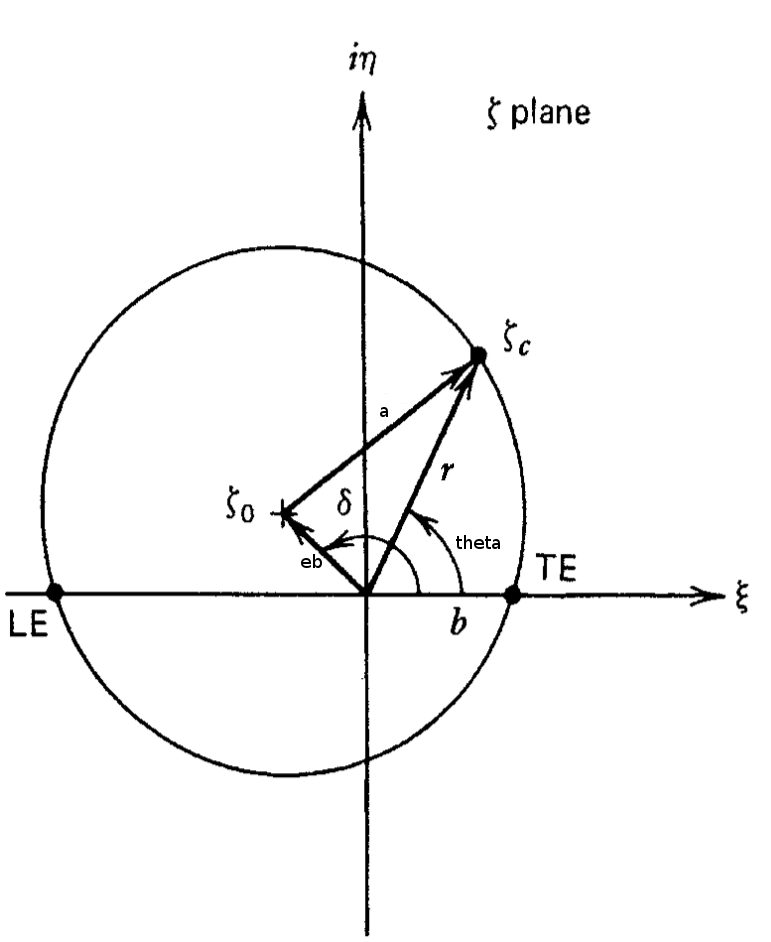
\includegraphics[scale=0.2]{./img/joukowski_cylinder.png}
    \caption{Cylinder in the $\zeta$ plane, i.e. the transformation domain. The cylinder if offset from the origin by $\zeta_0$}
    \label{joukowski_cylinder}
\end{figure}

\newpage
Let's start by defining the center of that cylinder.
\begin{equation}
    \zeta_0 = \epsilon b e^{i\delta} 
\end{equation}
The $\epsilon$ quantity is used to emphasize that the decentring needs to be ''small" so that the airfoil shape can be linearized, since a closed an explicit equation
for the full non linear airfoil is not known.
The cylinder points can be given by 
\begin{equation}
    \zeta_{c} =  r e^{i\theta} 
\end{equation}
From the cosine law  we can write $a$ length using two inscribed triangles in \ref{joukowski_cylinder} (note one of them isn't drawn).
\begin{align}
    a^2 &= (\epsilon b)^2 + r^2 - 2\epsilon b r \cos(\delta - \theta) \\
    a^2 &= (\epsilon b)^2 + b^2 - 2\epsilon b^2  \cos(\delta) 
\end{align}
Equating both equations 
\begin{align}
     (\epsilon b)^2 + r^2 - 2\epsilon b r \cos(\delta - \theta) &=  (\epsilon b)^2 + b^2 - 2\epsilon b^2  \cos(\delta)  \\
      r^2 - 2\epsilon b r \cos(\delta - \theta) &=   b^2 - 2\epsilon b^2  \cos(\delta) \\
      \left(\frac{r}{b}\right)^2 - 2\epsilon \frac{r}{b} \cos(\delta - \theta) &=   1 - 2\epsilon \cos(\delta) \\
      \left(\frac{r}{b}\right)^2 -  \left(\frac{r}{b}\right)2\epsilon \cos(\delta - \theta) -  1 + 2\epsilon \cos(\delta) &= 0
\end{align}
Solving for $r/b$.
\begin{align}
    \frac{r}{b} &= \frac{2\epsilon \cos(\delta - \theta) \pm \sqrt{4\epsilon^2 \cos^2(\delta - \theta)-4(  2\epsilon \cos(\delta)- 1)}} {2} \\
    \frac{r}{b} &= \epsilon \cos(\delta - \theta) \pm \sqrt{\epsilon^2 \cos^2(\delta - \theta)- 2\epsilon \cos(\delta)+ 1} \\
    \frac{r}{b} &= 1 + \epsilon \left( \cos(\delta -\theta) - \cos\delta \right) + \mathcal{O}[\epsilon^2]  \\
    \frac{r}{b} &= 1 + \epsilon \left( \sin\delta \sin\theta - \cos\delta \left(1 -\cos\theta \right) \right) + \mathcal{O}[\epsilon^2]  \\
    \frac{r}{b} &= 1 + \epsilon B + \mathcal{O}[\epsilon^2] \\
    r &\approx b\left(1 + \epsilon B \right)
\end{align}
To get the shape of the airfoil let us pass the circle coordinates through the Joukowski transform.
\begin{align}
    z_a &= \zeta_c + \frac{b^2}{\zeta_c}\\
    z_a &= re^{i\theta} + \frac{b^2}{re^{i\theta}}\\
    z_a &\approx b\left(1 + \epsilon B \right)e^{i\theta} + \frac{b^2}{b\left(1 + \epsilon B \right)}e^{-i\theta}\\
    z_a &\approx b\left(1 + \epsilon B \right)e^{i\theta} + b\frac{1}{1+\epsilon B}e^{-i\theta}
\end{align}
Developing in power series the last equation $\dfrac{1}{1+\epsilon B} =  1-\epsilon B + \mathcal{O}[\epsilon^2]$ .
\begin{align}
   z_a & \approx b\left(1+\epsilon B \right)e^{i\theta} + b\left(1-\epsilon B \right)e^{-i\theta} \\
   z_a & \approx b\left[ \left(1+\epsilon B\right)\left(\cos\theta + i\sin\theta \right) + \left(1-\epsilon B \right) \left(\cos\theta - i\sin\theta \right) \right]\\
   z_a & \approx b\left(  \cos\theta + i\sin\theta  +  \epsilon B\cos\theta + i\epsilon B\sin\theta +  \cos\theta - i\sin\theta    -\epsilon B\cos\theta + i\epsilon B\sin\theta \right)\\
   z_a & \approx 2b\left(\cos\theta +  i\epsilon B\sin\theta \right) \\
   z_a & \approx 2b\left(\cos\theta +  i\epsilon  \left( \sin\delta \sin^2\theta - \cos\delta \sin\theta\left(1 -\cos\theta \right) \right) \right)
\end{align}
The airfoil points in the  transformed plane $z_a= (x_a,y_a)$ are given by:
\begin{equation}
    \begin{dcases}
        x_a \approx 2b\cos\theta \\
        y_a \approx 2b\epsilon \left( \sin\delta \sin^2\theta - \cos\delta \sin\theta \left(1 -\cos\theta \right) \right) 
    \end{dcases}
    \label{airfoil_xy}
\end{equation}
The airfoil cord can be calculated has:
\begin{align}
    c &= z_a(\theta=0)-z_a(\theta=\pi) \\
    c &\approx 2b-(-2b) \nonumber \\
    c &\approx 4b \label{airfoil_cord}
\end{align}
Rewriting \eqref{airfoil_xy} in terms of the airfoil cord \eqref{airfoil_cord}.
\begin{equation}
    \begin{dcases}
        \bar{x}_a \defeq \frac{x_a}{c} \approx \frac{\cos\theta}{2} \\
        \bar{y}_a \defeq \frac{y_a}{c} \approx \frac{\epsilon}{2} \left( \sin\delta \sin^2\theta - \cos\delta \sin\theta \left(1 -\cos\theta \right) \right) 
    \end{dcases}
    \label{parametric_airfoil}
\end{equation}
It's possible do define an implicit equation for the airfoil shape, by replacing all the $\theta$ in the $y_a/c$ in equation \eqref{parametric_airfoil}, as variables of $x_a/c$ instead.
\begin{equation}
    \begin{dcases}
        \cos\theta = 2 \bar{x}_a  \quad \vee \quad \sin\theta = \pm \sqrt{1 - 4\bar{x}_a^2} \\
        \bar{y}_a  = \frac{\epsilon}{2}\sin\delta \left( 1 - 4\bar{x}_a^2 \right) \pm \frac{\epsilon}{2} \cos\delta \sqrt{1 - 4\bar{x}_a^2} \left(1 -2\bar{x}_a\right) 
    \end{dcases}
    \label{implicit_airfoil}
\end{equation}
The linearized Joukowski airfoil given by \eqref{implicit_airfoil} can be understood as a camber contribution plus a thickness contribution applies on the upper or lower camber line.
\begin{align}
    \bar{y}_a = \underbrace{\frac{\epsilon}{2}\sin\delta \left( 1 - 4\bar{x}_a^2 \right)}_\textrm{Camber Line}\notate[X]{{}\pm{}}{2}{\parbox[t]{3in}{\scriptsize $+$Upper, $-$Lower airfoil }}  
                \underbrace{\frac{\epsilon}{2} \cos\delta  \left(1 -2\bar{x}_a\right)\sqrt{1 - 4\bar{x}_a^2}}_\textrm{Thickness Distribution} 
    \label{linear_joukowski_airfoil}                
\end{align}
Calculating the maximum of the camber line of \eqref{linear_joukowski_airfoil}.
\begin{align}
    \bar{y}_c = \frac{\epsilon}{2}\sin\delta \left( 1 - 4\bar{x}_a^2 \right) \\
    \frac{h}{c} \defeq \left(\bar{y}_c \right)_{max} \Leftrightarrow \frac{d\bar{y}_c}{d\bar{x}_a} = 0 \\
    \frac{d\bar{y}_c}{d\bar{x}_a} =  \frac{d}{d\bar{x}_a}\left(  \frac{\epsilon}{2}\sin\delta \left( 1 - 4\bar{x}_a^2 \right) \right) = 0 \\
    \frac{\epsilon}{2}\sin\delta \left( 0 - 8\bar{x}_a \right) = 0 \\
    \bar{x}_a = 0 \\
    \bar{h} \defeq \frac{h}{c} = \frac{\epsilon}{2}\sin\delta 
\end{align}

% \section{NACA Airfoils}
% The National Advisory Committee for Aeronautics (NACA) the predecessor for NASA, led in the early 1930 and 1940 an intensive research program on airfoil development. 
% Several families of airfoils where developed, each with advantages on some aerodynamic conditions. One thing in common across NACA airfoil families/series is the 
% digit nomenclature, for example the `n' series has `n' digits that assign `n' parameters to that airfoil family, like maximum thickness, lift coefficient or cord location 
% of the maximum pressure coefficient, etc.

% \newpage
% \subsection{NACA 4-Series}
% NACA d\textsubscript{1}d\textsubscript{2}d\textsubscript{3}d\textsubscript{4}%$d_1d_2d_3d_4$

% \begin{description}[align=left,labelwidth=1cm]
% \item [d\textsubscript{1}] maximum relative camber $f/c$ in percentage.
% \item [d\textsubscript{2}] $(x/c)_{f/c}$ position of maximum camber, in tenths of cord.
% \item [d\textsubscript{3}d\textsubscript{4}] percentage of relative thickness $t/c$
% \end{description}

% The shape of the airfoil is given by the analytical definition of the upper $(x_u,y_u)$ and lower $(x_l,y_l)$  points of it's surface.
% \begin{align}
%     x_u &= x - y_t\sin(\theta) \\
%     y_u &= y_c + y_t\sin(\theta)\\
%     x_l &= x + y_t\sin(\theta) \\
%     y_l &= y_c - y_t\sin(\theta)
% \end{align}
% For this cambered airfoil, because the thickness needs to be applied perpendicular to the camber line, the coordinates 

% The thickness height $y_t$ is given by
% \begin{equation}
%     \frac{y_t}{c} = \frac{(d_3d_4)}{100} \left[ 1.4845\left(\frac{x}{c} \right)^{\frac{1}{2}} - 0.63\left(\frac{x}{c} \right) -  1.758\left(\frac{x}{c} \right)^2 +  1.4215\left(\frac{x}{c} \right)^3 - 0.5075\left(\frac{x}{c} \right)^4  \right]
% \end{equation}

% The camber height $y_c$ is given consists of two parabola arches that intersect at the point of maximum camber $((x/c)_{f/c}, f/c) = (d_2, d_1)$
% \begin{align}
%     \frac{y_c}{c} &= \frac{d_1}{d_2^2} \left(\frac{x}{c}\right)\left[ 2d_2 -\left(\frac{x}{c}\right)\right] \qquad  &0& \leq \left(\frac{x}{c}\right) \leq d_2\\
%     \frac{y_c}{c} &= \frac{d_1}{(1-d_2)^2} \left[1- 2d_2 + 2d_2\left(\frac{x}{c}\right) -\left(\frac{x}{c}\right)^2\right] \qquad &d_2 \leq \left(\frac{x}{c}\right) \leq 1
% \end{align}





\newpage
\chapter{Wing Theory}
Lets start by defining a few geometric quantities useful in wing theory.
\begin{equation}
    \label{cord_am}
    \bar{\bar{c}} = \frac{1}{S} \int\limits_{-b/2}^{b/2} c^2 dy
\end{equation}

\begin{equation}
    \label{cord_sm}
    \bar{c} = \frac{S}{b} 
\end{equation}


\begin{equation}
    \label{aspect_ration}
    \AR = \frac{b}{\bar{c}} 
\end{equation}

\section{Lifting Line Theory}





